


%% ─── SLIDE 1: Study Area & Data ───────────────────────────────────────────
\begin{frame}{ Data}

\begin{itemize}[label=\textbullet]
    \item We use soil texture data from Germany. The data comes from the 2018 LUCAS survey.
    
    \vspace{0.5em}
    
    \item We have around 1,785 observations. Each observation contains three components: clay, sand, and silt — and together they always sum to one, which makes this compositional data.
    

  
    
    \vspace{0.5em}
    
    \item A total of \textbf{133 environmental covariates} (at $250 \times 250$ m resolution) were used as predictors, including climate, temperature, and vegetation-related variables.
    
    \vspace{0.5em}
   
\end{itemize}

\end{frame}


% %% ─── SLIDE 2: Spatial Patterns ─────────────────────────────────────────────
% \begin{frame}{Spatial Distribution of Soil Texture}

% \begin{figure}
%     \centering
%     \begin{columns}
%         \begin{column}{0.33\textwidth}
%             \centering
%             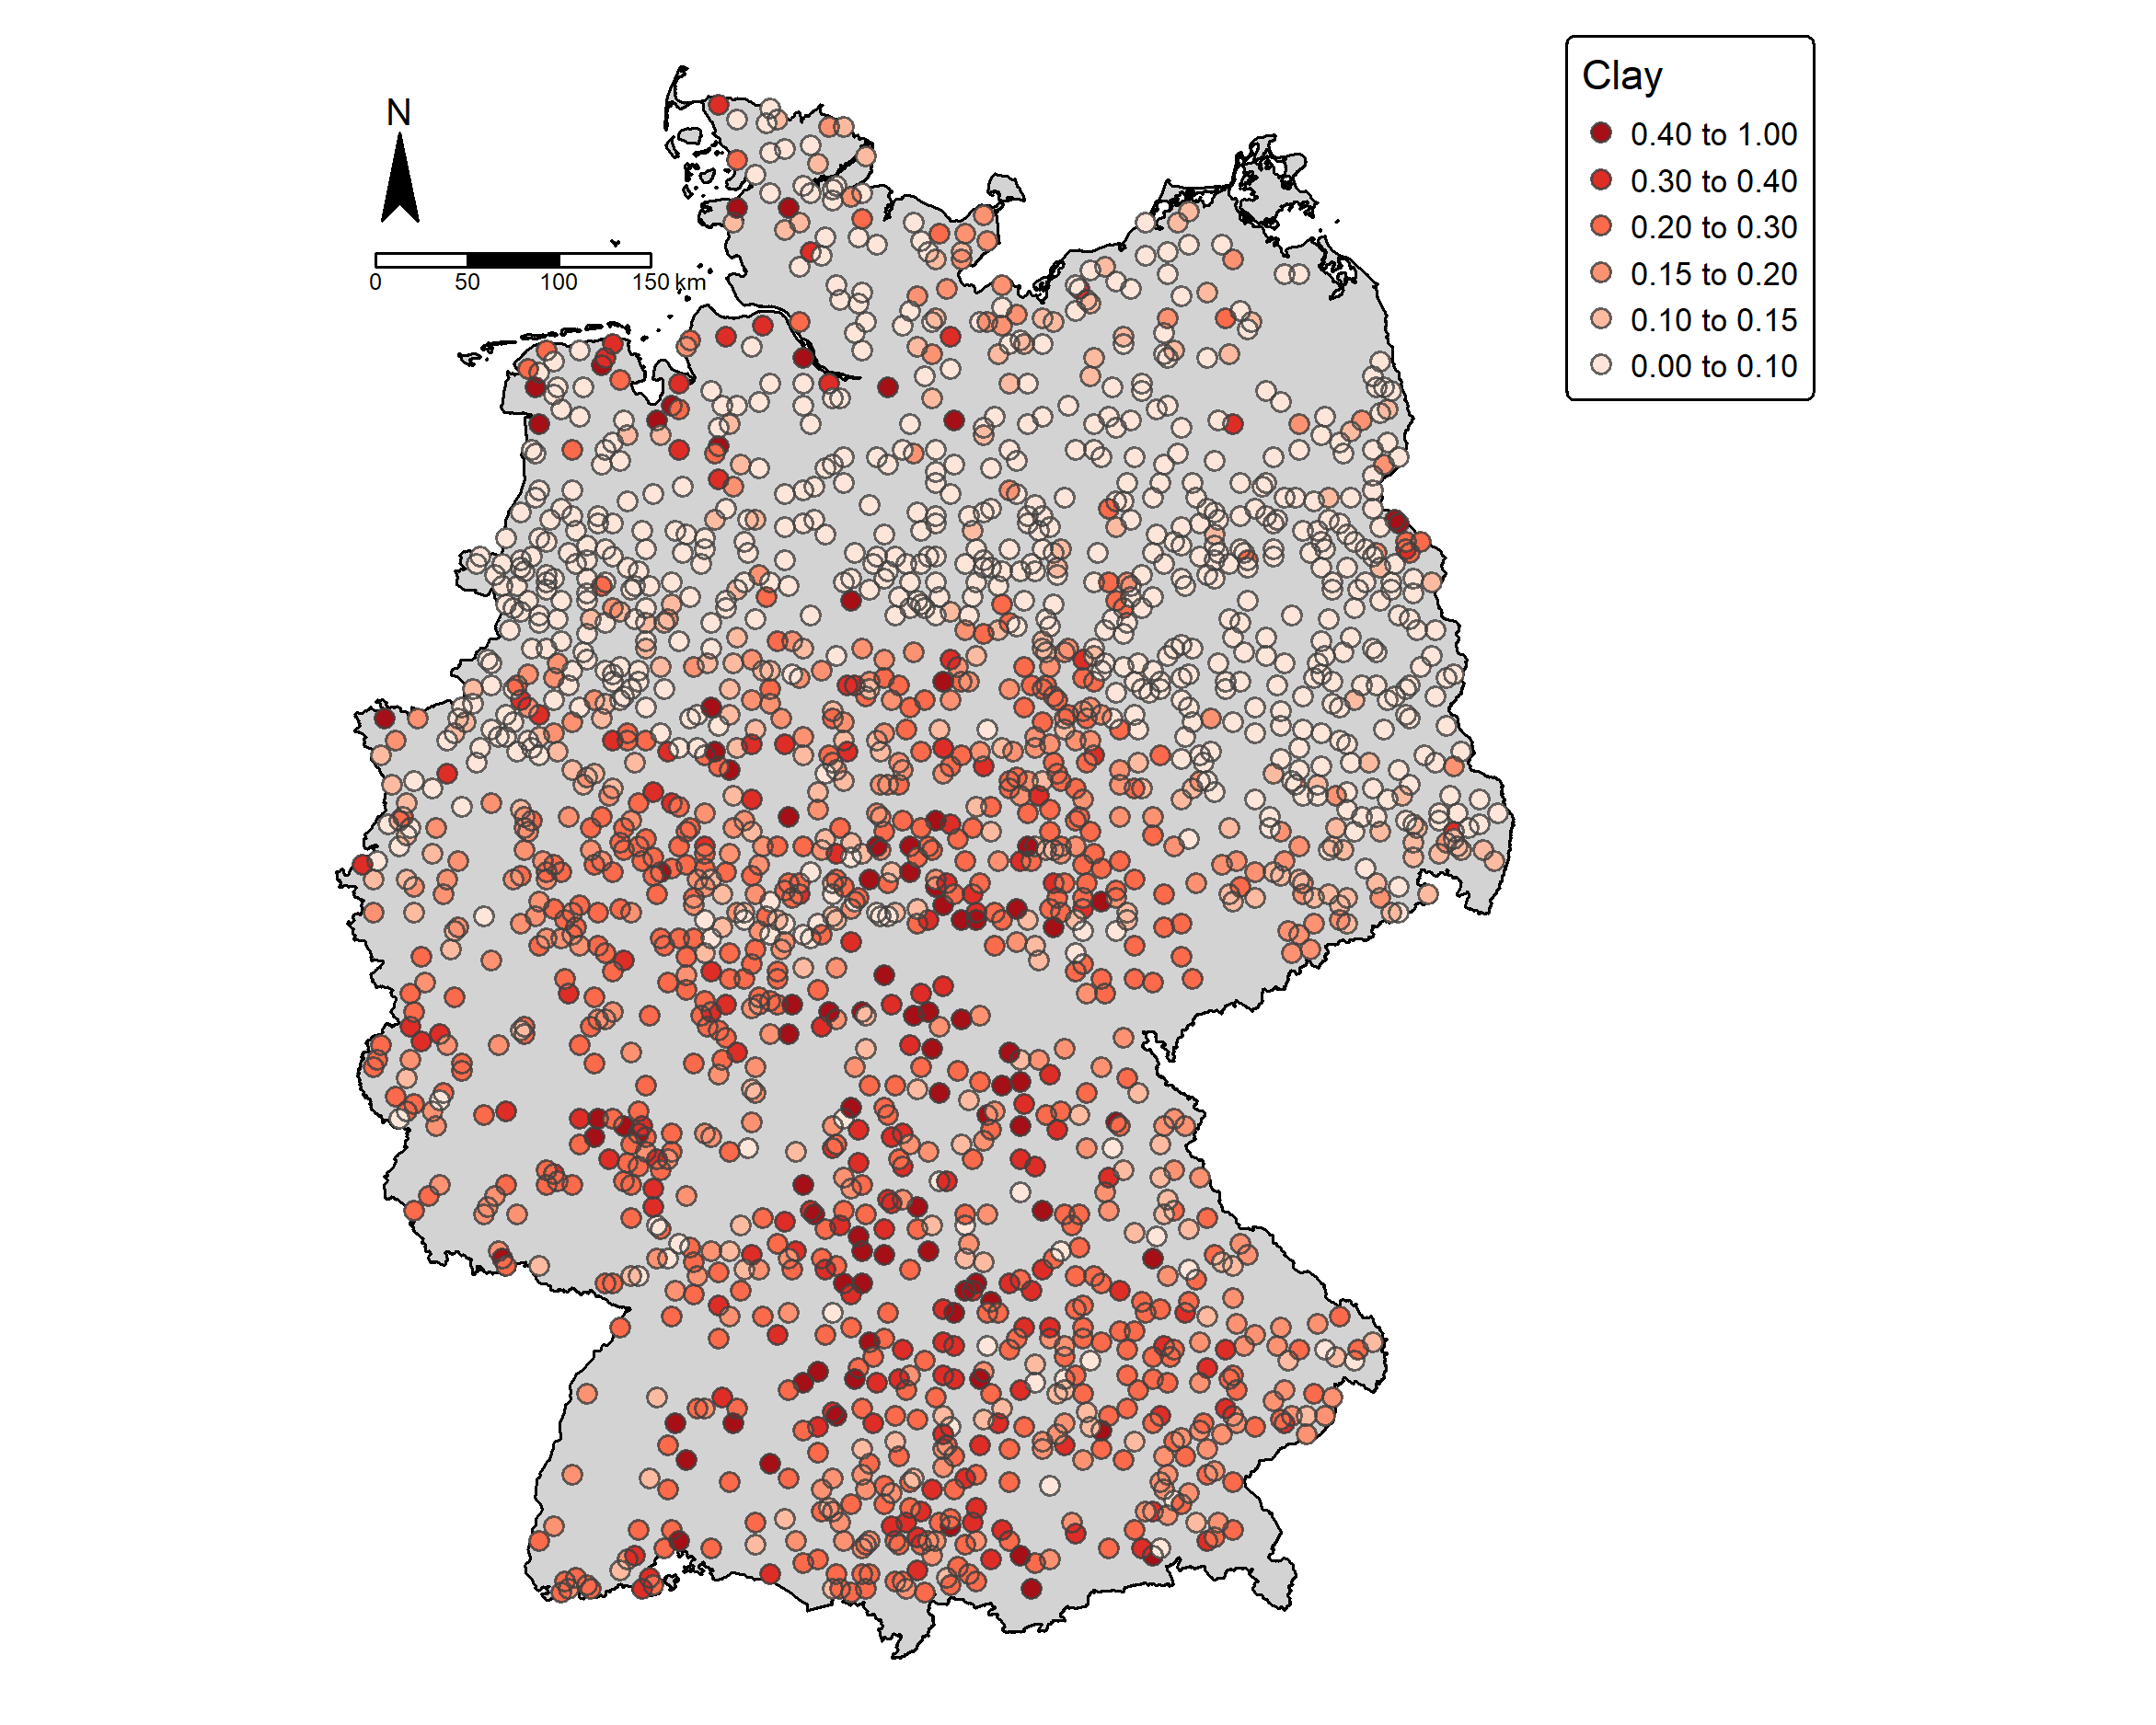
\includegraphics[width=\linewidth]{Figures/pointmap_clay.png}
%             \\ (a) Clay
%         \end{column}
%         \begin{column}{0.33\textwidth}
%             \centering
%             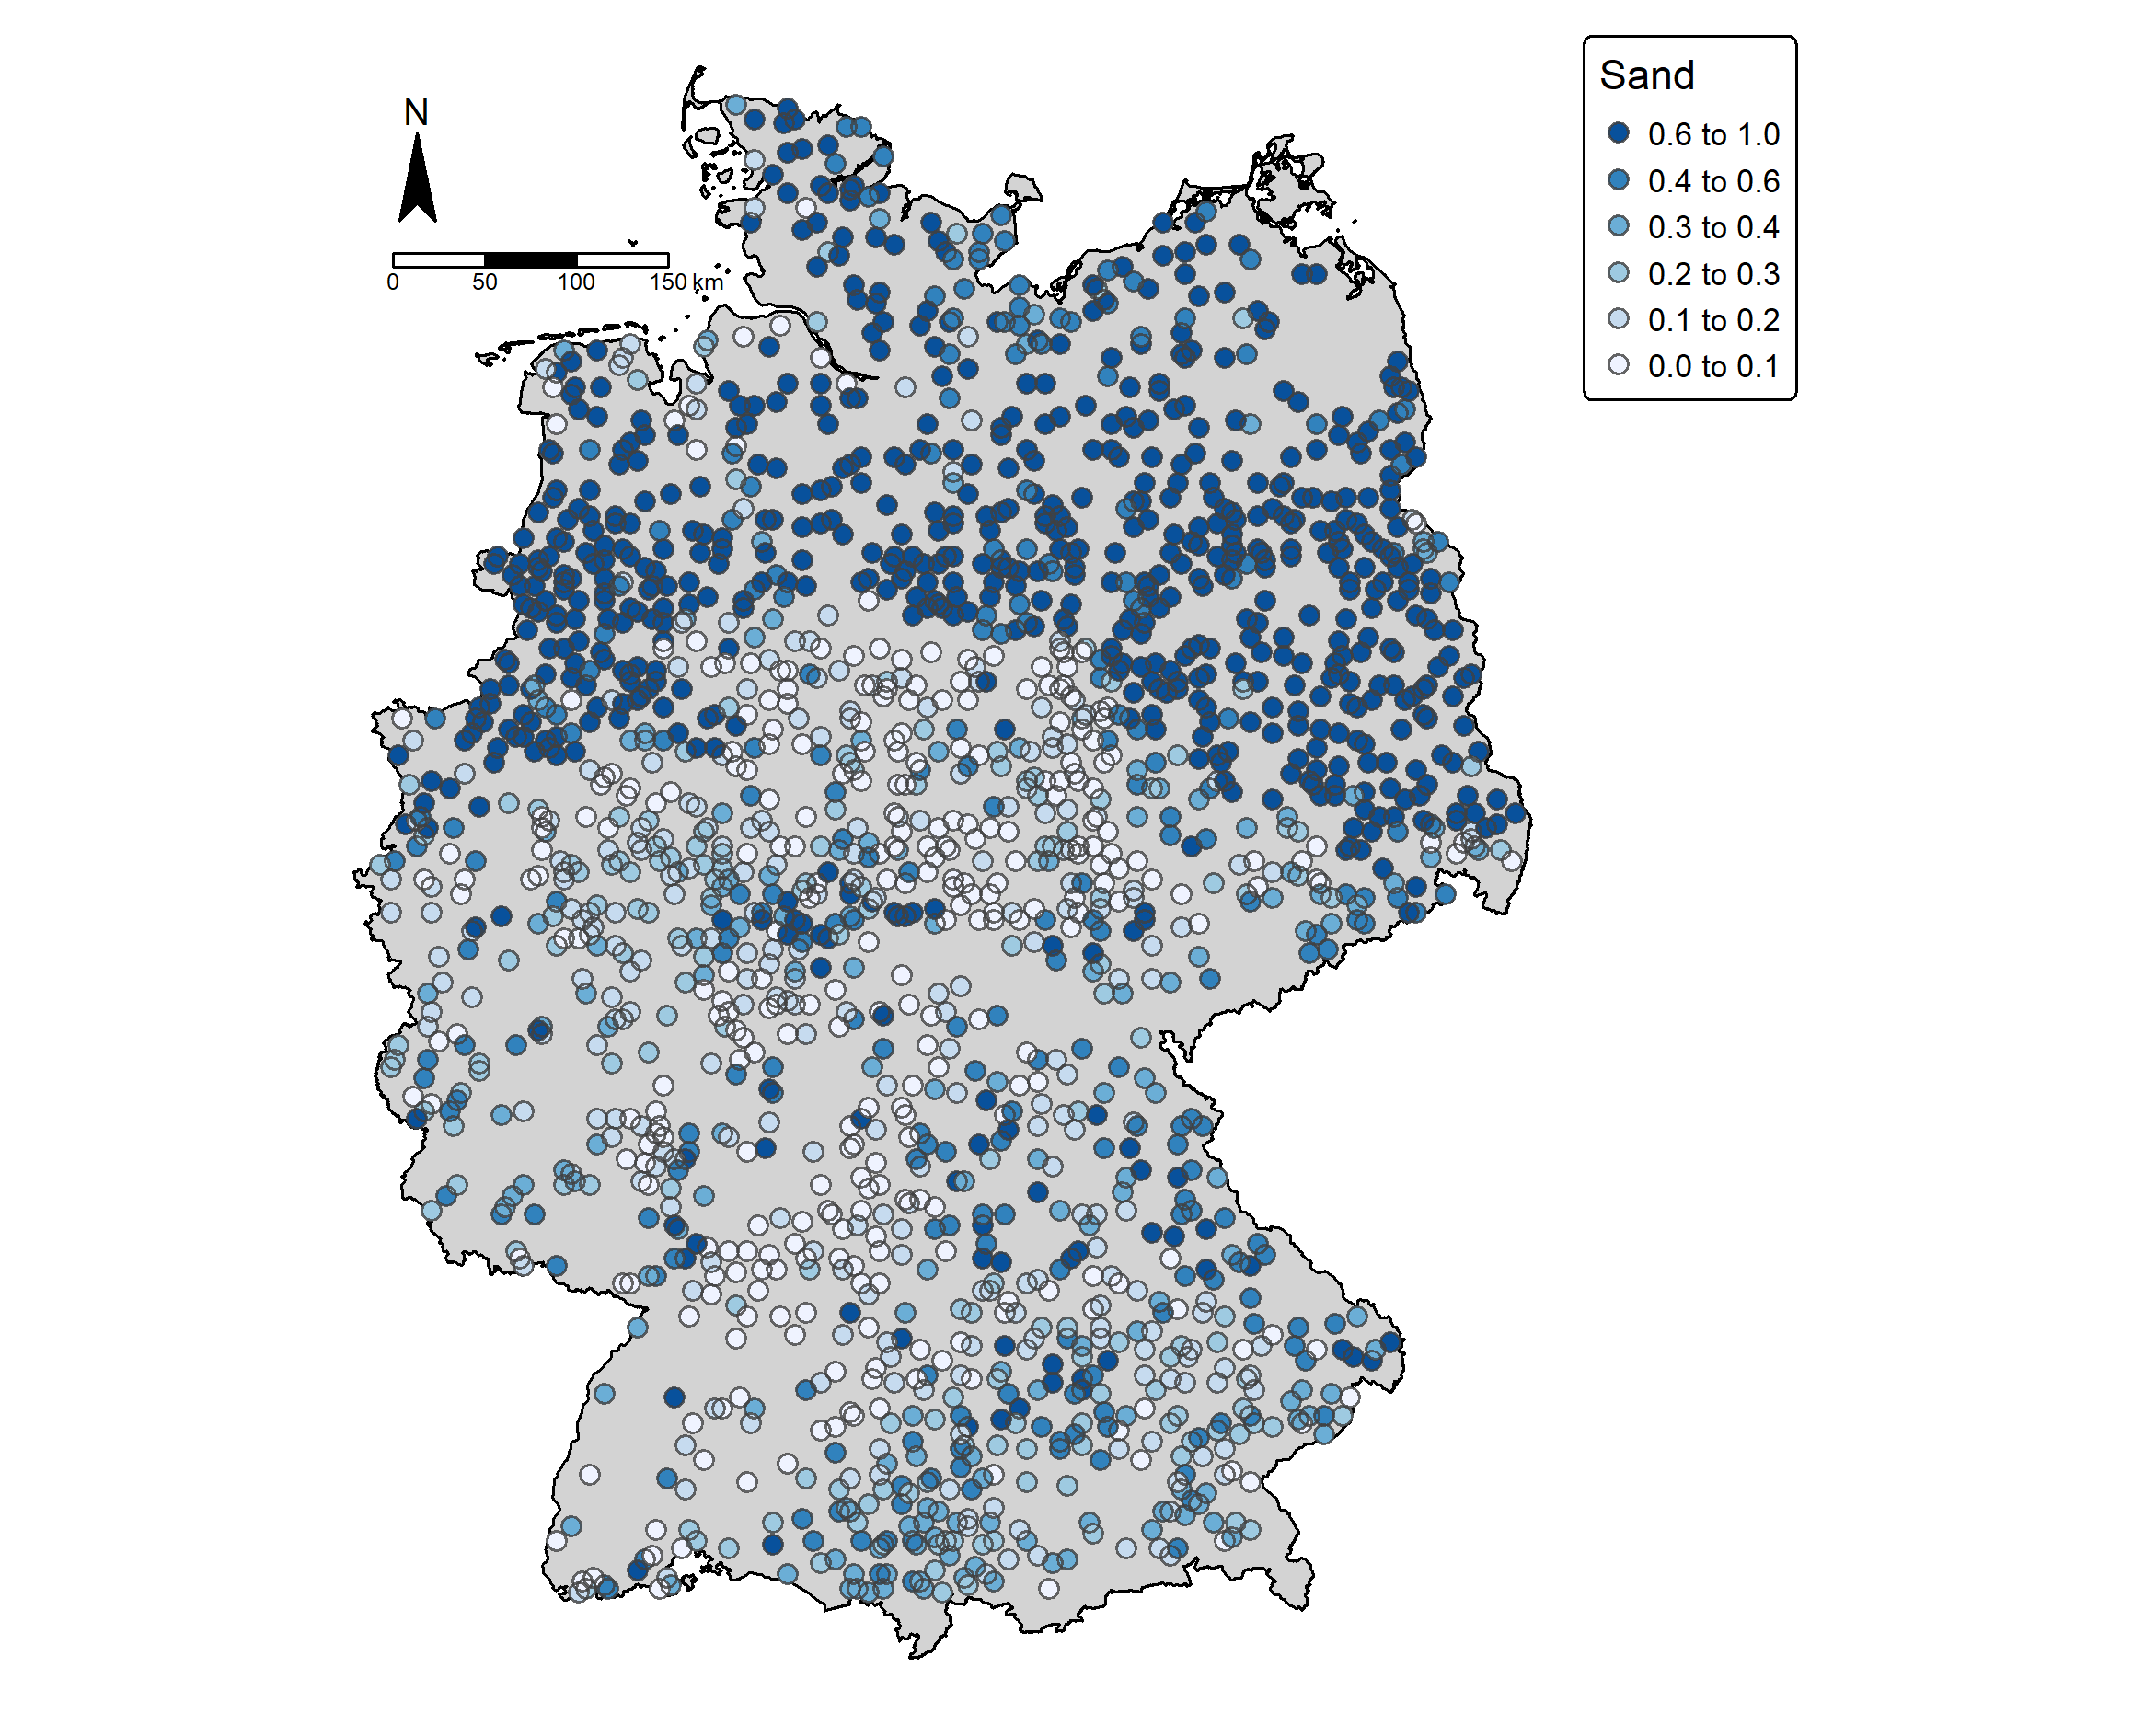
\includegraphics[width=\linewidth]{Figures/pointmap_sand.png}
%             \\ (b) Sand
%         \end{column}
%         \begin{column}{0.33\textwidth}
%             \centering
%             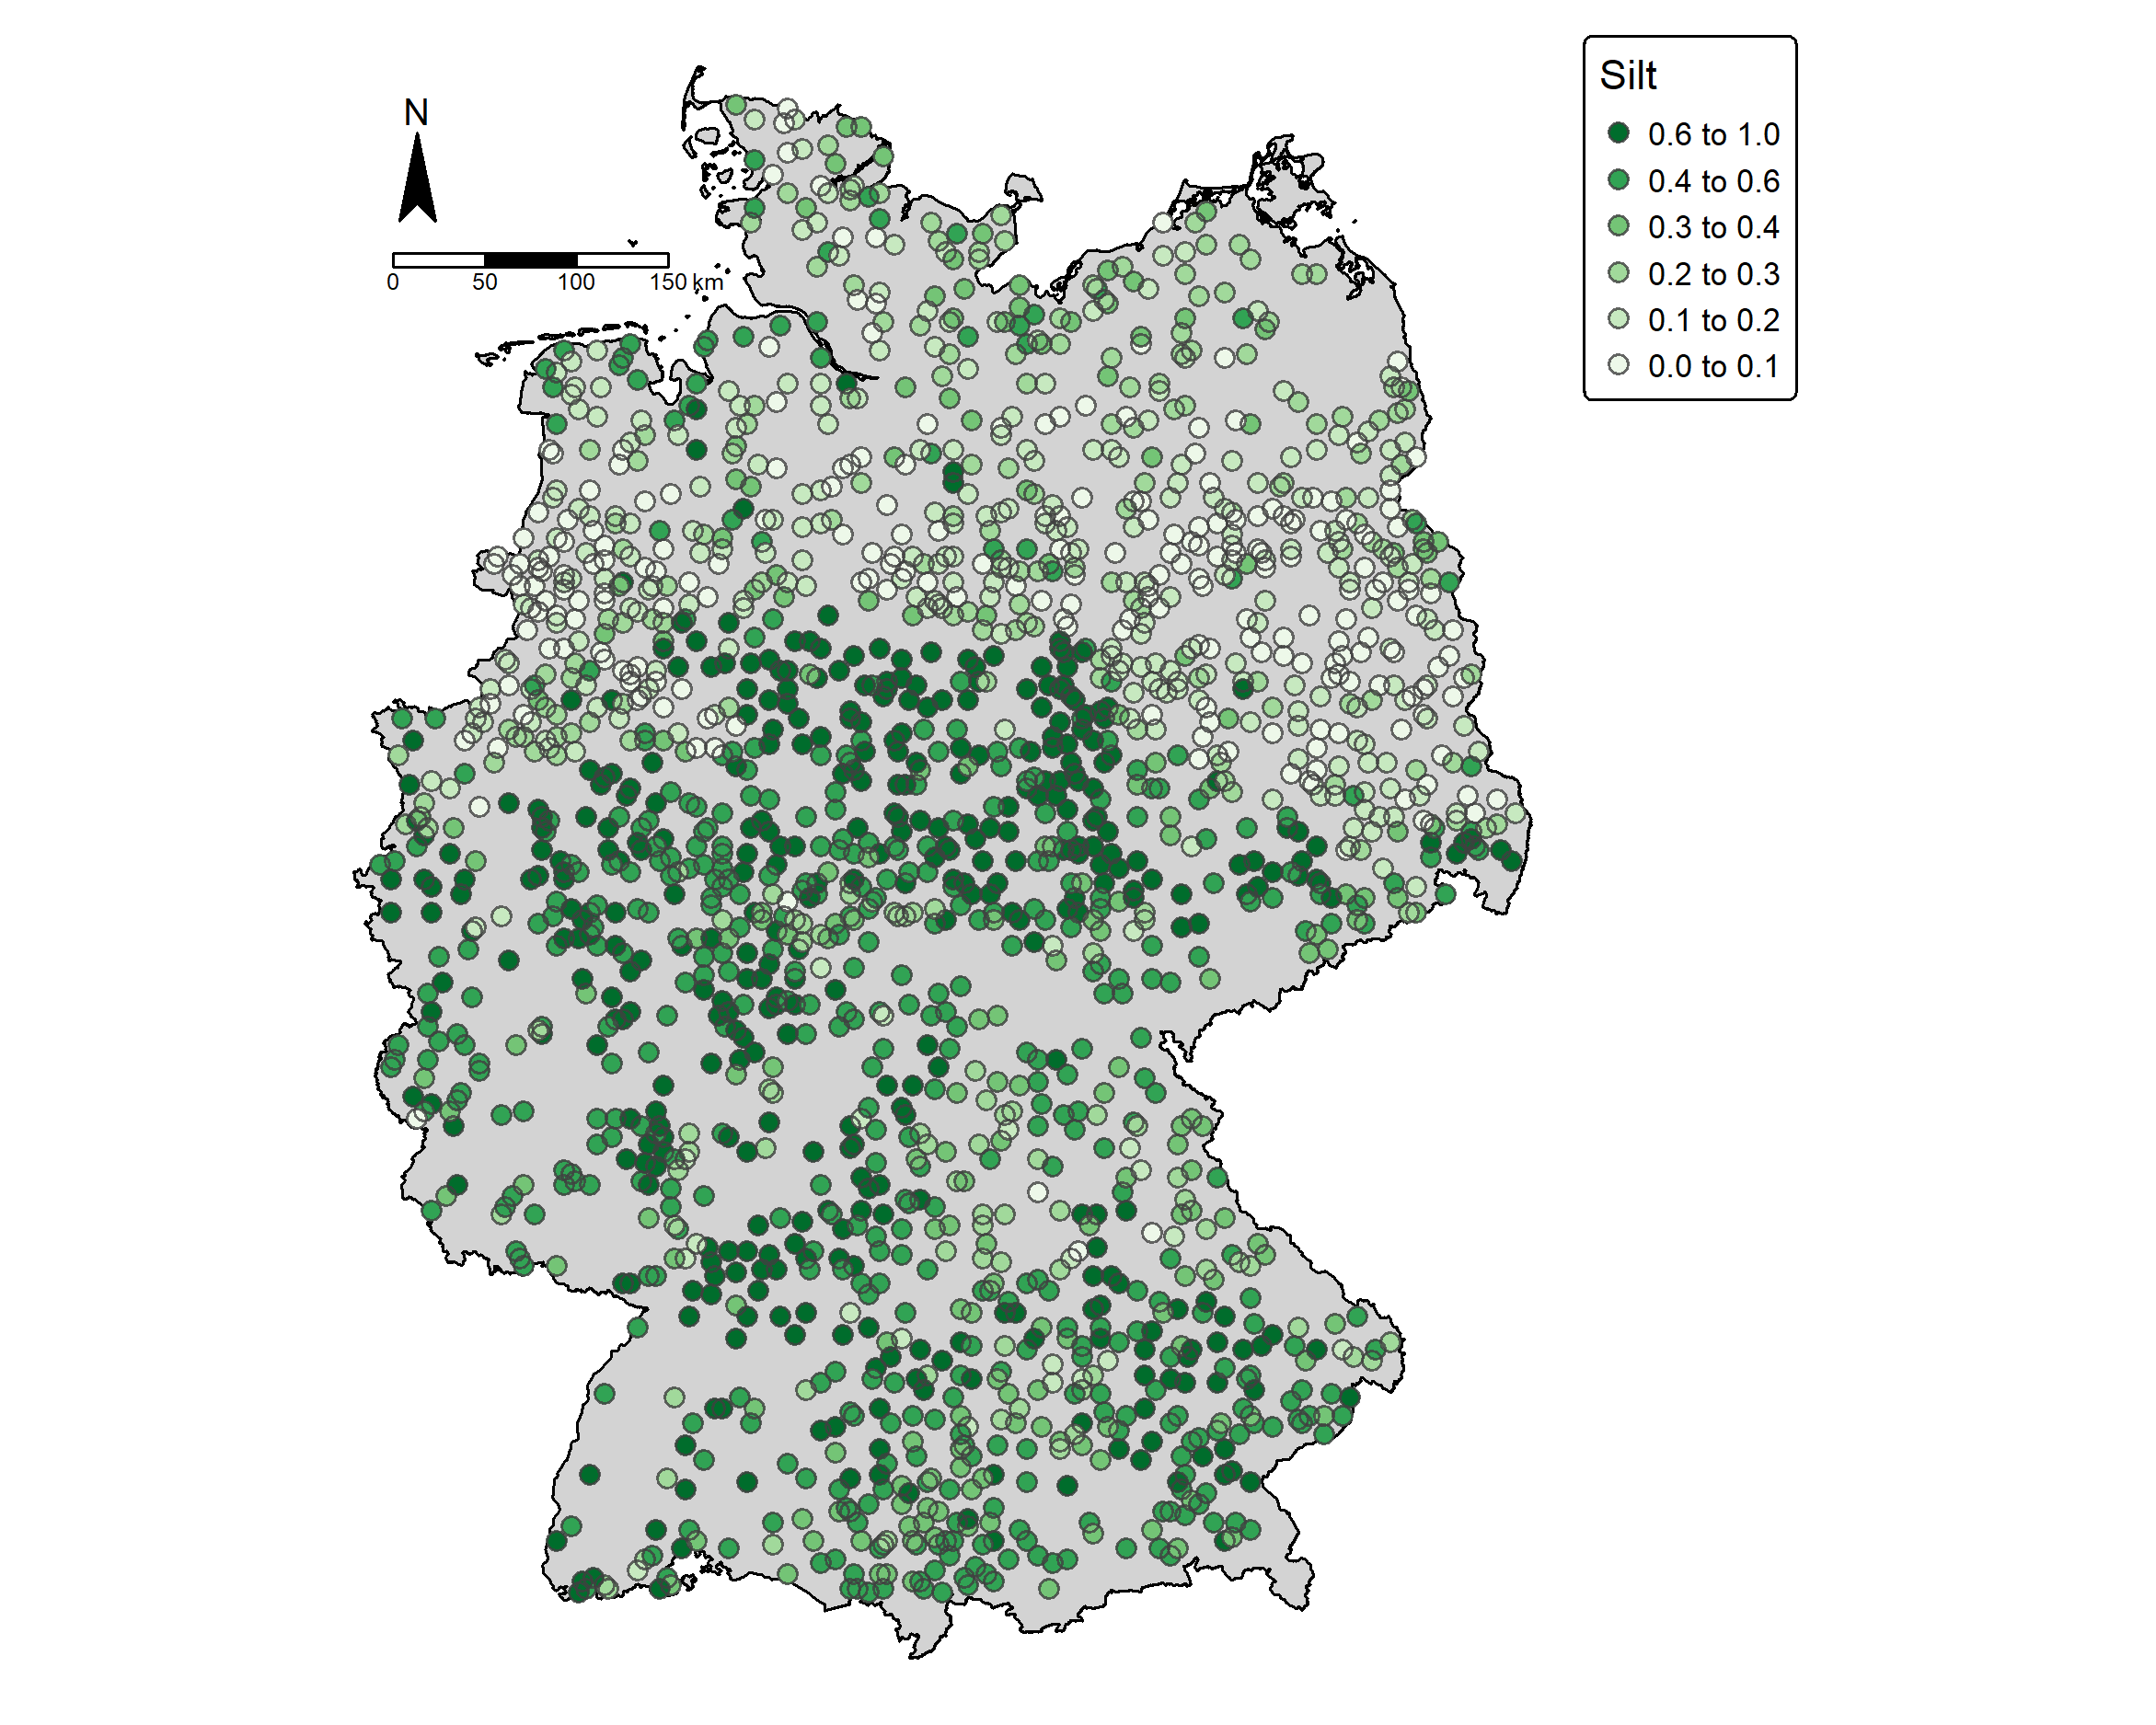
\includegraphics[width=\linewidth]{Figures/pointmap_silt.png}
%             \\ (c) Silt
%         \end{column}
%     \end{columns}
%     \caption{LUCAS soil texture observation locations in Germany: (a) Clay, (b) Sand, (c) Silt (shown as proportions).}
% \end{figure}

% \end{frame}

%% ─── SLIDE 2: Spatial Patterns ─────────────────────────────────────────────
\begin{frame}{Spatial Distribution of Soil Texture}

\begin{columns}

    \begin{column}{0.45\textwidth}
        \begin{itemize}
            \item[1.] Each point represents one \textbf{observation location} in Germany.
            
            \item[2.] The \textbf{colour} of each point indicates the value of the component: darker colours indicate \textbf{higher values}, lighter colours indicate \textbf{lower values}.
            
            \item[3.] \textbf{Clay:} higher values concentrated in the \textbf{south and centre}.
            
            \item[5.] \textbf{Sand:} higher values mostly in the \textbf{north and north-east}.
            
            \item[6.] \textbf{Silt:} more mixed pattern, with elevated values across the \textbf{central belt}.
        \end{itemize}
    \end{column}

    \begin{column}{0.55\textwidth}
        \only<1>{
        \begin{figure}
            \centering
            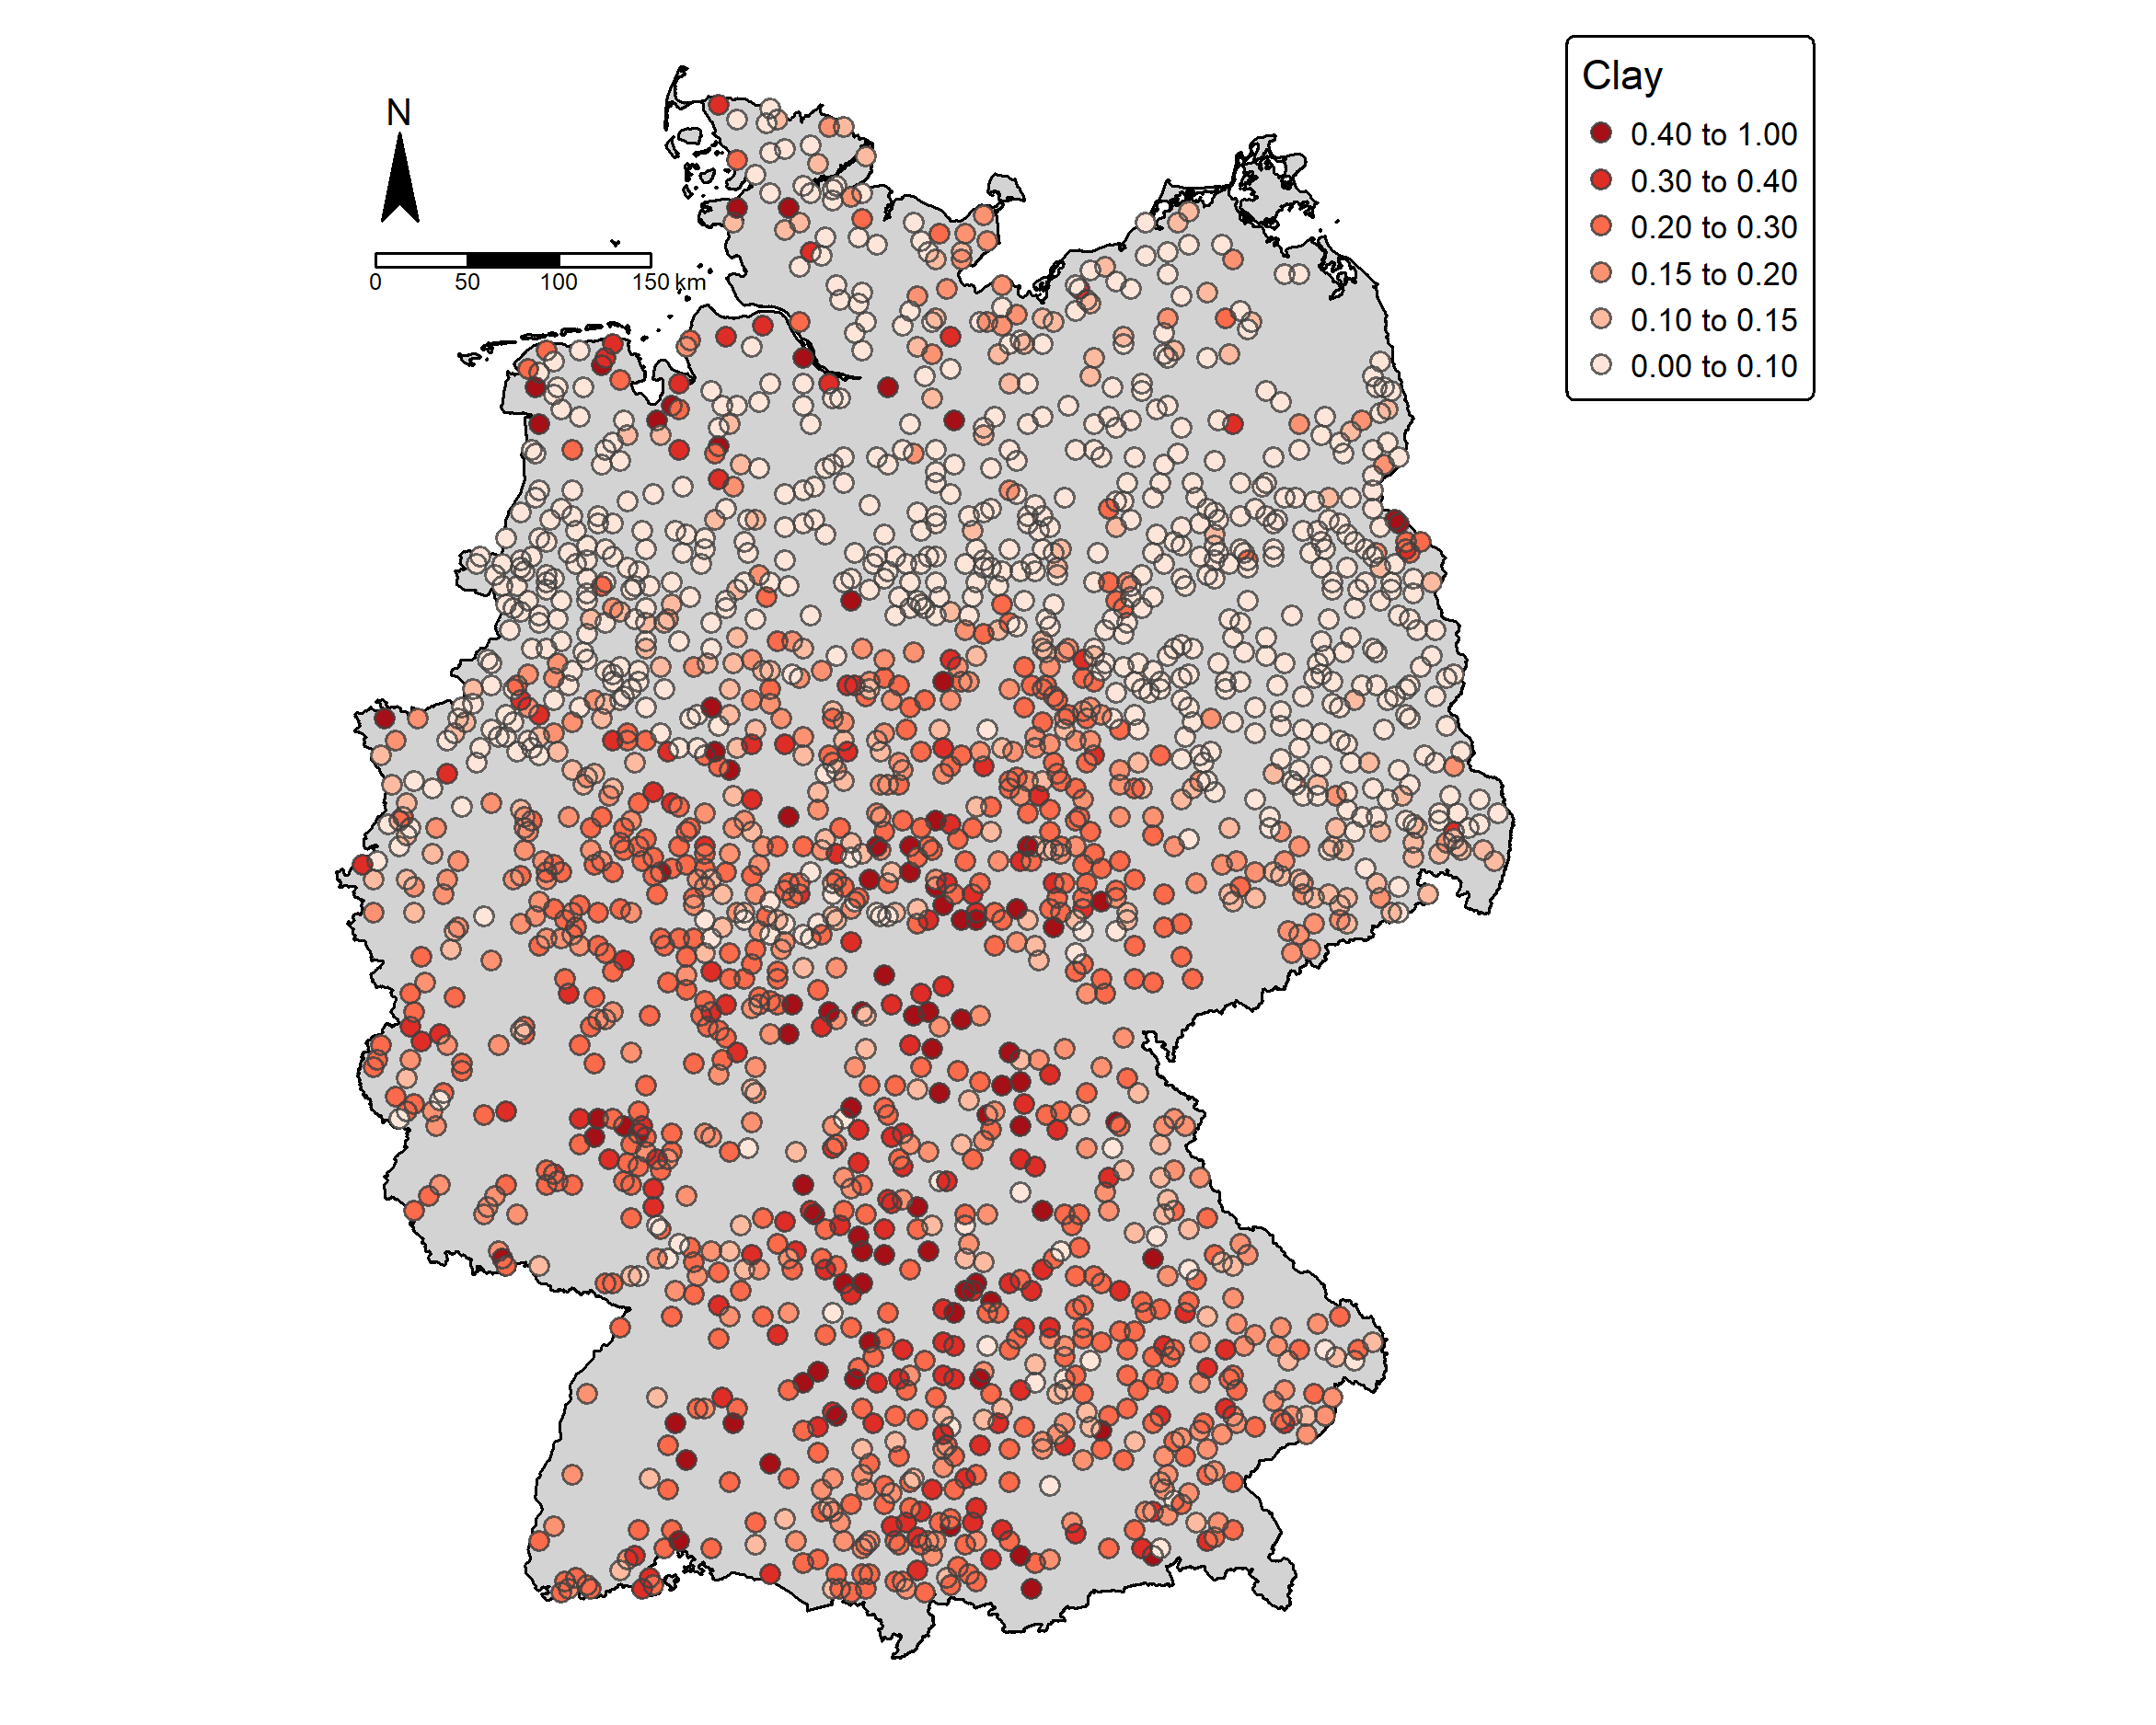
\includegraphics[width=\linewidth]{Figures/pointmap_clay.png}
            \caption{LUCAS soil texture observation locations in Germany: Clay.}
        \end{figure}}
        \only<2>{
        \begin{figure}
            \centering
            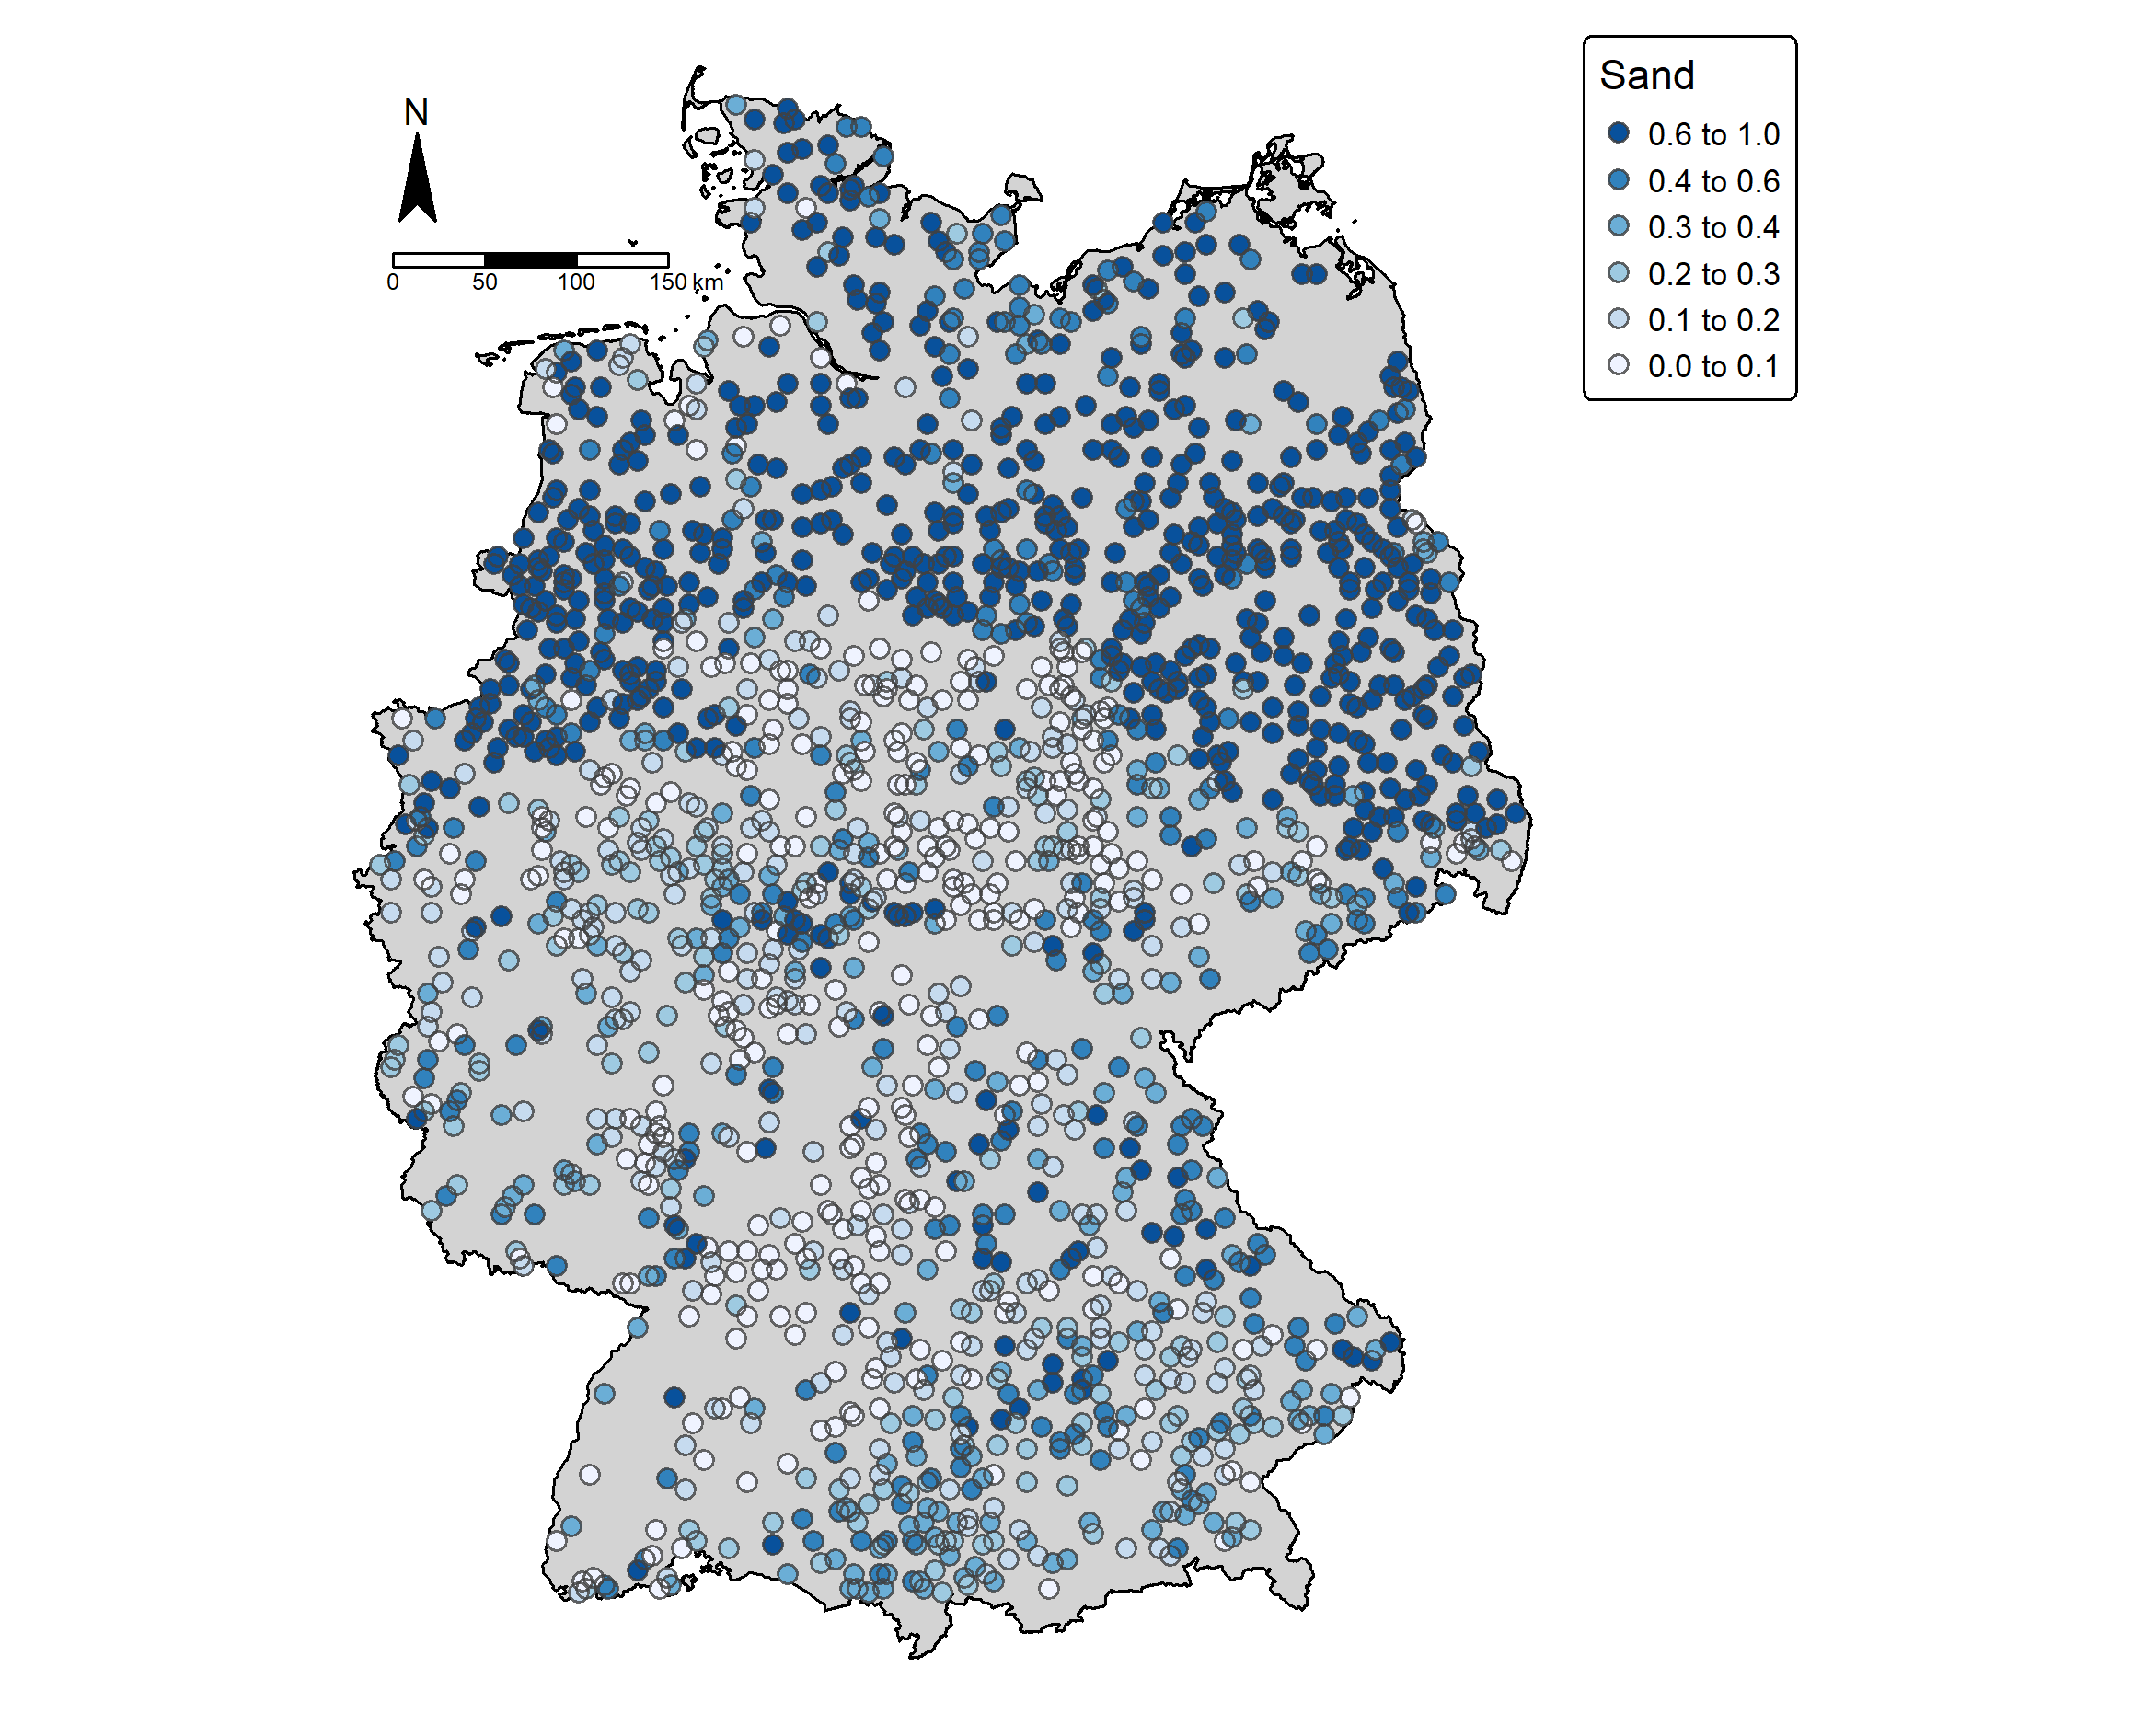
\includegraphics[width=\linewidth]{Figures/pointmap_sand.png}
            \caption{LUCAS soil texture observation locations in Germany: Sand.}
        \end{figure}}
        \only<3>{
        \begin{figure}
            \centering
            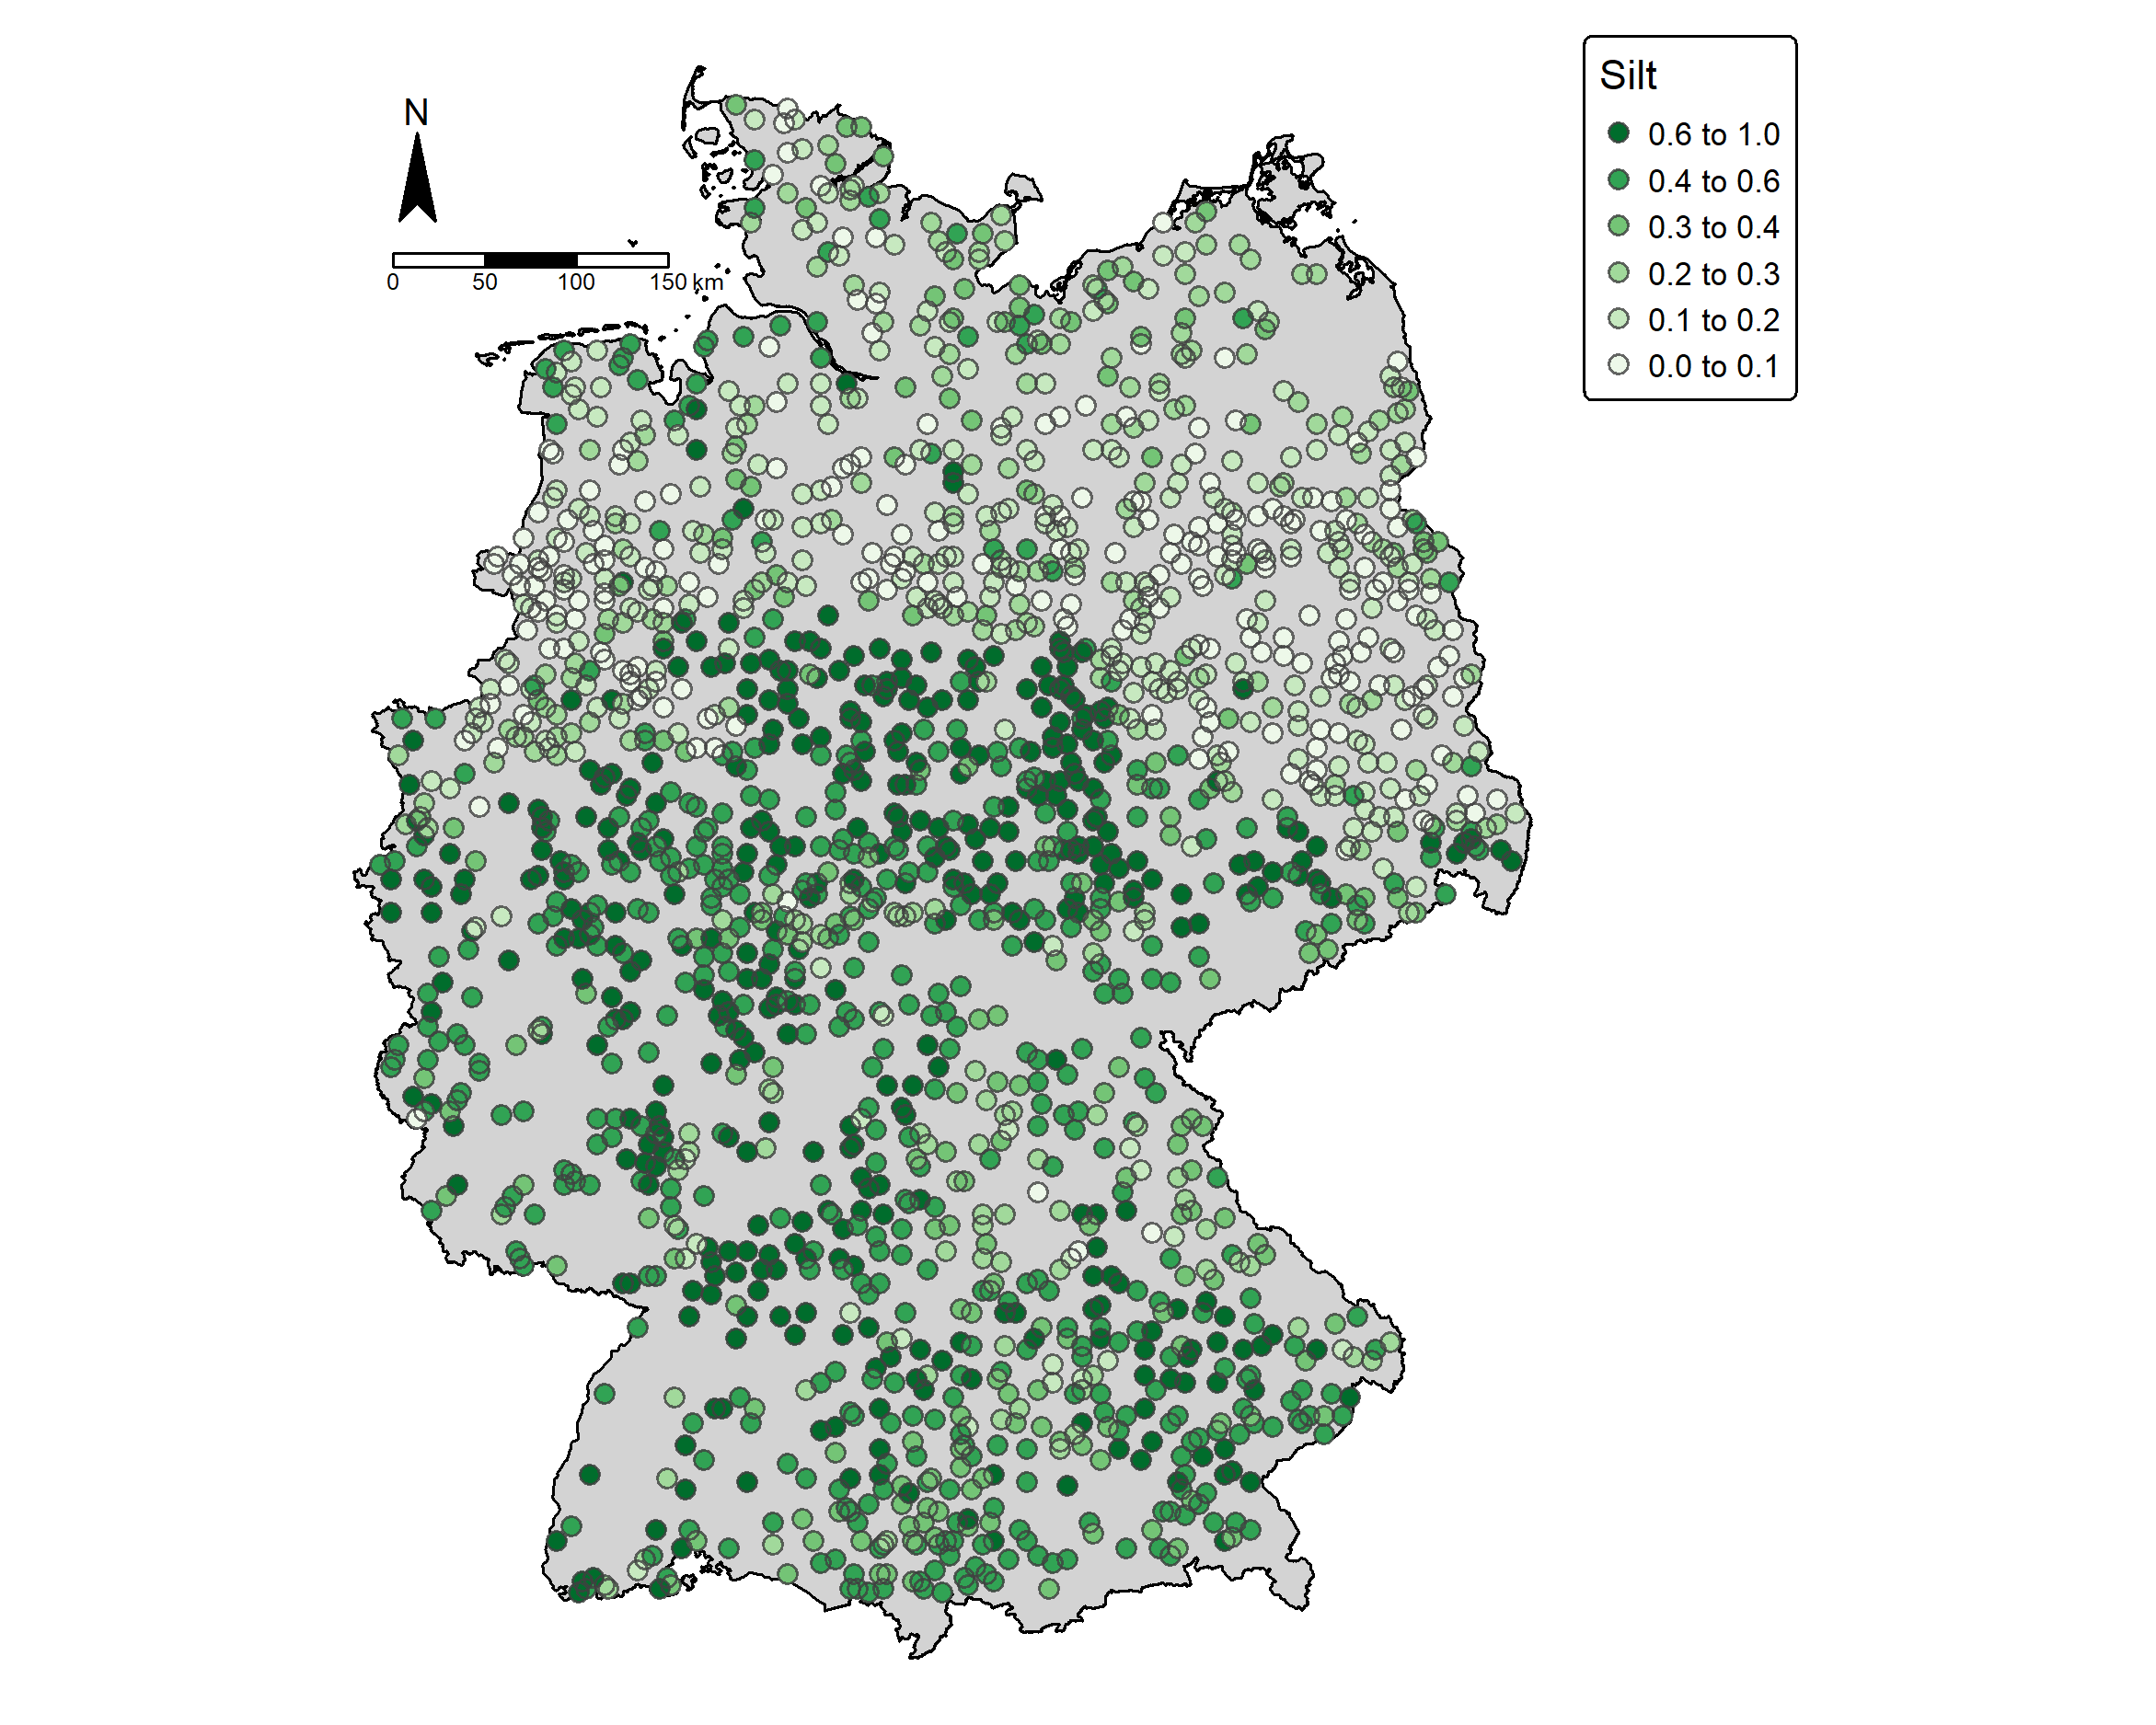
\includegraphics[width=\linewidth]{Figures/pointmap_silt.png}
            \caption{LUCAS soil texture observation locations in Germany: Silt.}
        \end{figure}}
    \end{column}

\end{columns}

\end{frame}

\begin{frame}{Ternary Plot of Soil Texture}

\begin{columns}

    \begin{column}{0.45\textwidth}
        \begin{itemize}
            \item[1.] A \textbf{ternary plot} is a triangle where each corner represents $100\%$ of one component: clay, sand, or silt.

           
            
            \item[2.] Points closer to a corner have a \textbf{higher proportion} of that component.

            \item[3.] Most observations cluster along the \textbf{sand--silt} edge, meaning few samples have high clay content.

            \item[4.] The spread of points reflects the \textbf{large variability} of sand and silt compared to clay.
        \end{itemize}
    \end{column}

    \begin{column}{0.55\textwidth}
        \begin{figure}
            \centering
            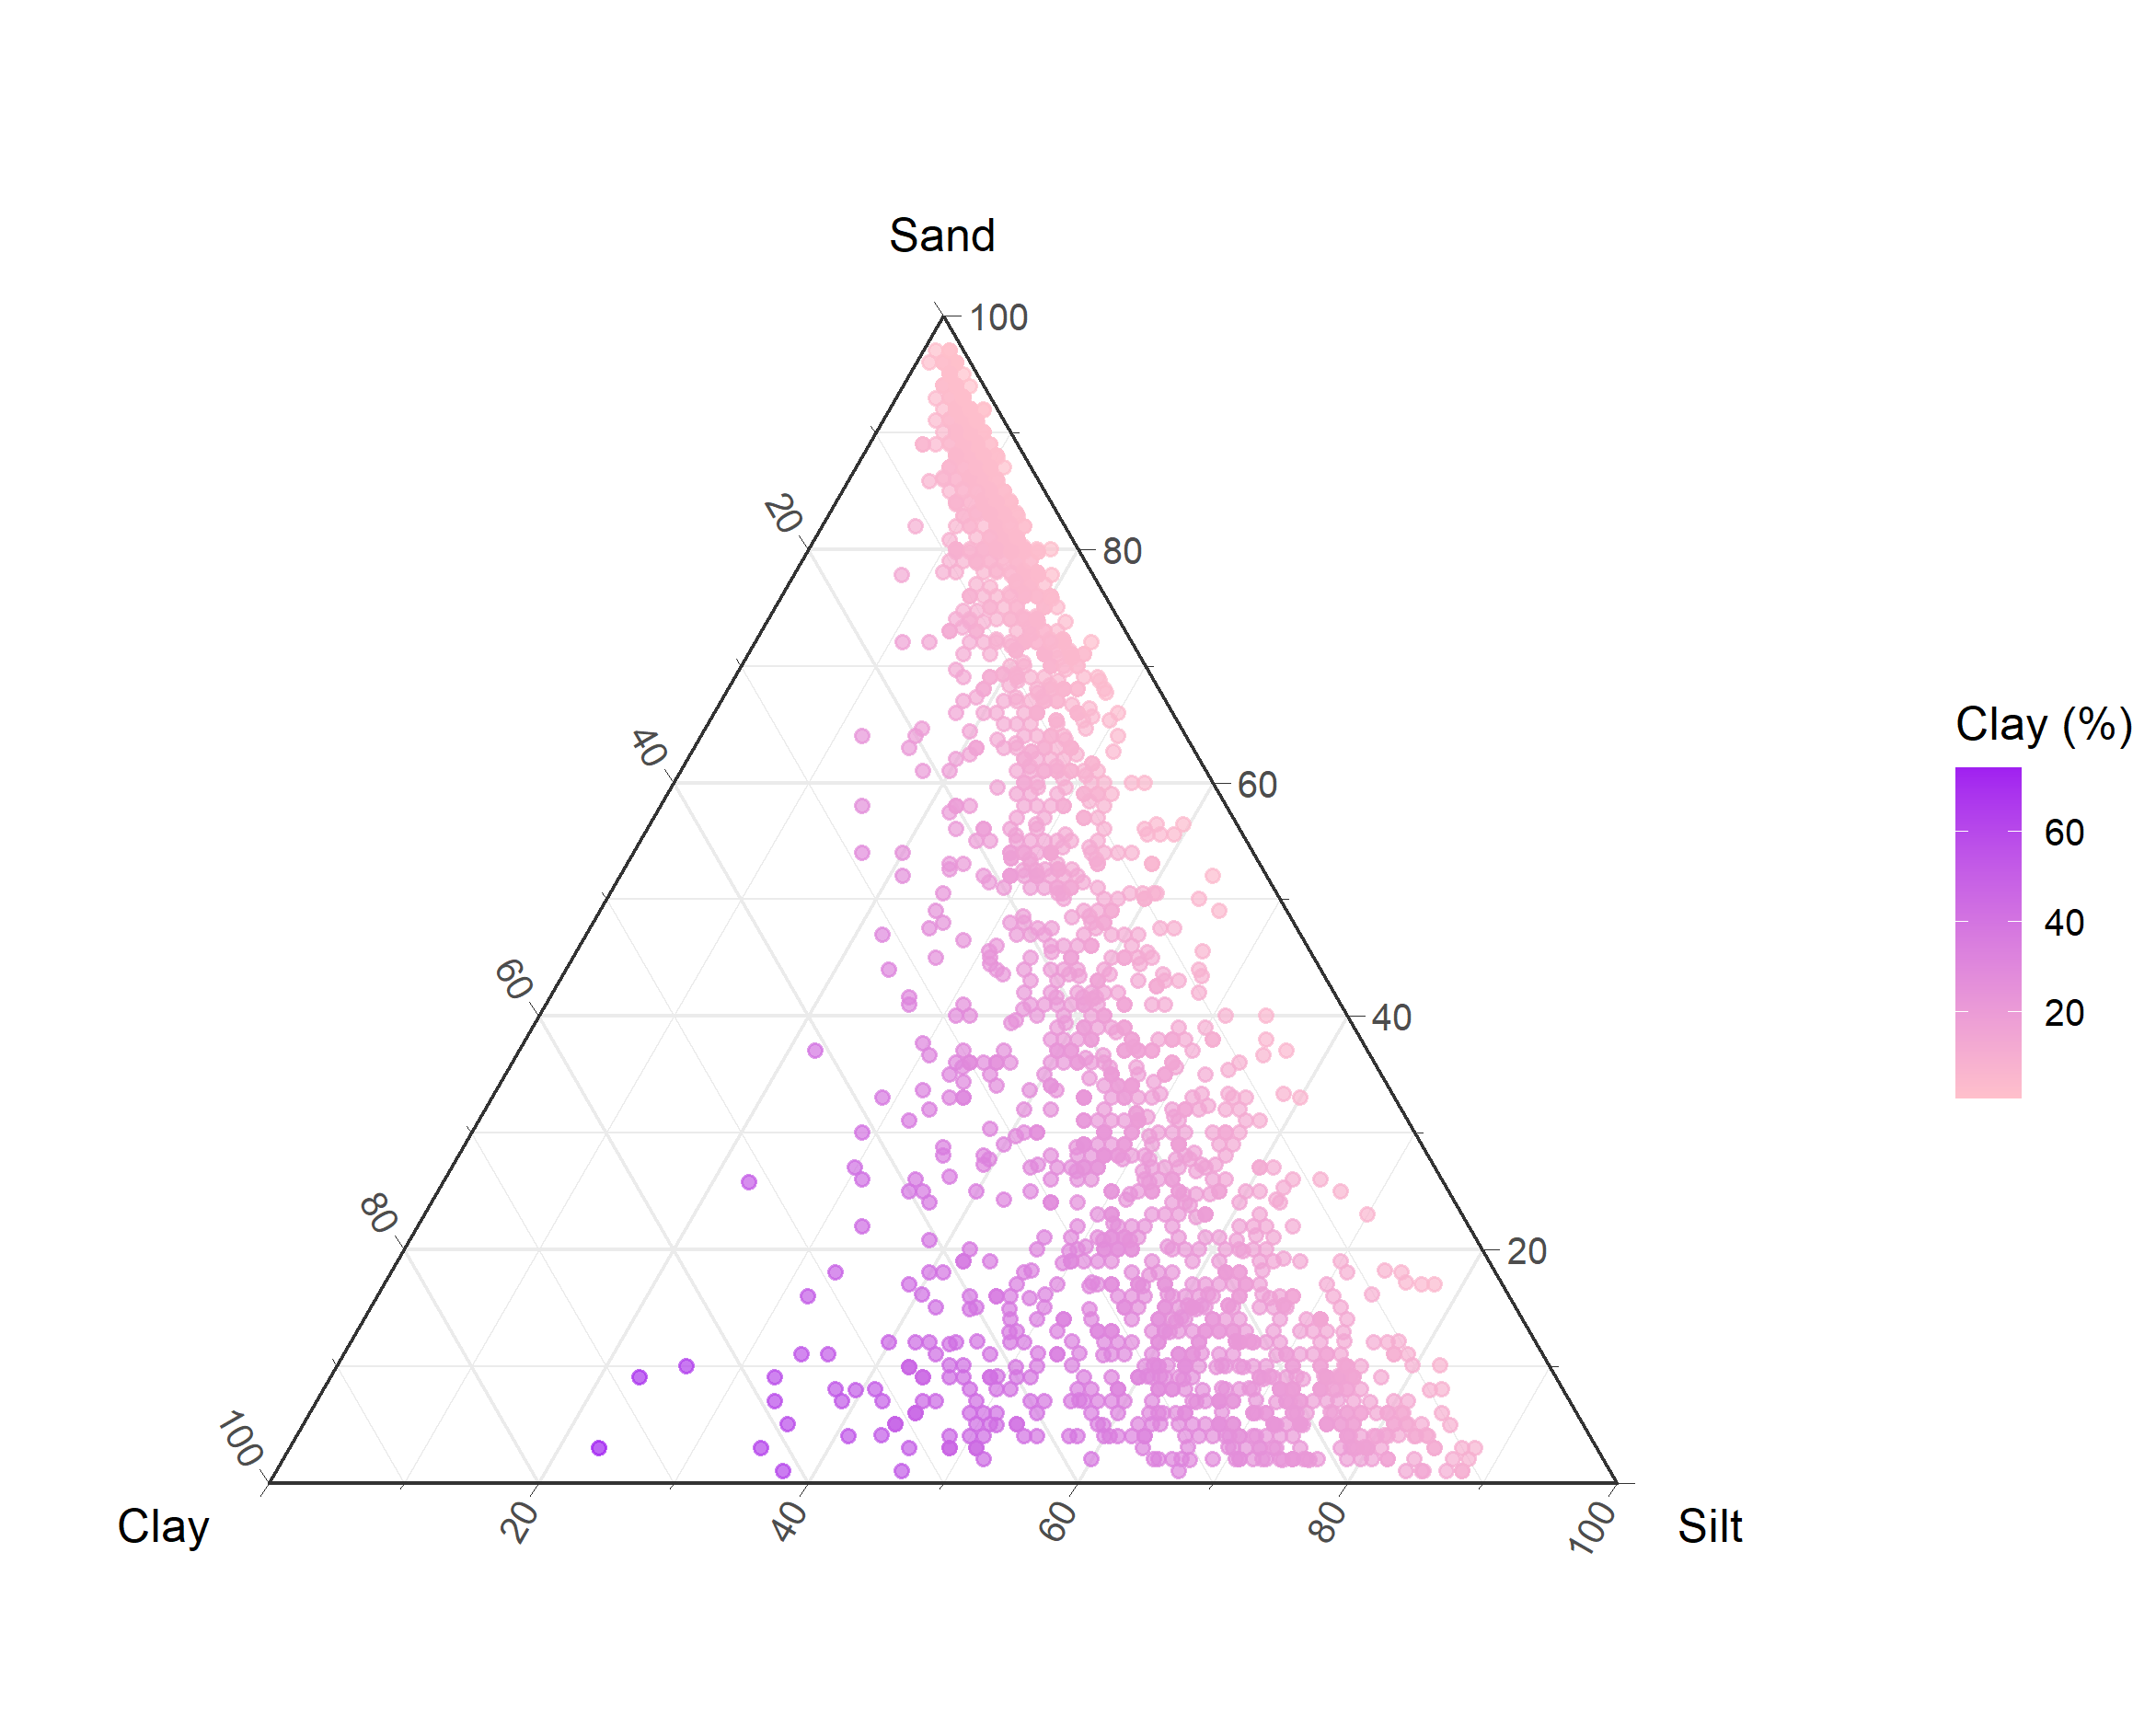
\includegraphics[width=\linewidth]{Figures/point_tern.png}
            \caption{Ternary plot of clay, sand, and silt distributions.}
        \end{figure}
    \end{column}

\end{columns}

\end{frame}

%% ─── SLIDE 4: Modelling Strategies ─────────────────────────────────────────
\begin{frame}{Modelling Strategies}

Five modelling approaches were compared:

\begin{table}
\centering
\small
\begin{tabular}{lccc}
\toprule
Model & Joint estimation & Respects geometry & Transformation \\
\midrule
RF (raw)         & No  & No  & No  \\
MRF (raw)        & Yes & No  & No  \\
ilr-RF           & No  & Yes & Yes \\
ilr-MRF          & Yes & Yes & Yes \\
\textbf{DirichletRF}   & Yes & Yes & No  \\
\bottomrule
\end{tabular}
\caption{Summary of modelling strategies.}
\end{table}

\begin{itemize}
    \item RF and MRF on raw components serve as \textbf{baseline} approaches.
    \item \textbf{DirichletRF} works directly on the simplex without requiring any log-ratio transformation.
\end{itemize}

\end{frame}




%% ─── SLIDE 4: Modelling Strategies ─────────────────────────────────────────
\begin{frame}{Evaluation Metrics}

To compare these models, we used  the Aitchison Distance and the Root Mean Square Error, or RMSE.
\vspace{0.2cm}
\textbf{1. Aitchison Distance:}
\[
AC = \frac{1}{n} \sum_{i=1}^n \sqrt{\sum_{j=1}^k \left(\log\frac{Y_{ij}}{g(\mathbf{Y}_i)} - \log\frac{\hat{Y}_{ij}}{g(\hat{\mathbf{Y}}_i)}\right)^2},
\]
\[
\text{where} \quad g(\mathbf{Y}_i) = \left(\prod_{j=1}^k Y_{ij}\right)^{1/k}
\]
\textit{Measures compositional dissimilarity using log-ratio geometry.}

\vspace{0.3cm}
\textbf{2. Root Mean Square Error (RMSE):}
$
\text{RMSE}_k =  \sqrt{\frac{1}{n} \sum_{i=1}^n (Y_{ij} - \hat{Y}_{ij})^2}
$

\vspace{0.3cm}
\textbf{Interpretation:} Lower values for both metrics indicate better predictive accuracy.
\end{frame}



\begin{frame}{Parameter Tuning and Cross-Validation}

\begin{itemize}
    \item[1.] All models were assessed using \textbf{10-fold nested cross-validation},
    with the same folds shared across methods to ensure a fair comparison.

    \item[2.]  Each random forest model was fitted with \textbf{500 trees}.

    \item[3.]  Hyper-parameters were selected by grid search:
    \begin{itemize}
        \item[3.1]  minimum node size: $\{2, 5, 10\}$
        \item[3.2] $m_{\mathrm{try}}$: $\{23, 29, 35, 41, 47, 53, 59, 65\}$
    \end{itemize}

    \item[4.] For \textbf{DirichletRF}, minimum node size was fixed at 5 for computational efficiency.

    \item[5.] Performance was quantified using \textbf{RMSE} and \textbf{Aitchison distance}.

    \item[6.] For the  comparison, models were refitted on the full dataset using
    the best hyper-parameters from the inner folds.
\end{itemize}

\end{frame}




%% ─── SLIDE 6: Results ───────────────────────────────────────────────────────
\begin{frame}{Results: RMSE and Aitchison Distance}

\begin{table}
\centering
\small
\caption{RMSE and Aitchison Distance (AC) across modelling approaches.}
\begin{tabular}{lccccc}
\toprule
 & RF & ilr-RF & MRF & ilr-MRF & \textbf{DirichletRF} \\
\midrule
\multicolumn{6}{c}{\textbf{RMSE}} \\
\midrule
Clay        & 0.086 & 0.086 & 0.088 & 0.087 & \textbf{0.085} \\
Sand        & 0.186 & 0.181 & 0.188 & 0.182 & \textbf{0.168} \\
Silt        & 0.148 & 0.145 & 0.150 & 0.146 & \textbf{0.135} \\
Aggregated  & 0.140 & 0.137 & 0.142 & 0.138 & \textbf{0.130} \\
\midrule
\multicolumn{6}{c}{\textbf{Aitchison Distance (AC)}} \\
\midrule
AC & 0.852 & 0.788 & 0.861 & 0.798 & \textbf{0.766} \\
\bottomrule
\end{tabular}
\end{table}

\begin{itemize}
    \item \textbf{DirichletRF} achieves the lowest RMSE across all components and the smallest AC.
    \item The largest gains are observed for \textbf{sand} and \textbf{silt}.
    \item ilr-based models only marginally outperform their untransformed counterparts.
\end{itemize}

\end{frame}


%% ─── FRAME 1: Cross-Validation Explanation ──────────────────────────────────
\begin{frame}{Publication}

\begin{center}
\vfill

\begin{block}{}
\begin{center}
\textbf{Dirichlet Random Forest for Predicting Compositional Data}\\[0.4em]
\end{center}
\end{block}

\vspace{0.5em}

\textbf{Authors:}\\[0.3em]
\underline{Masoumifard, K.}, van der Westhuizen, S., Gardner-Lubbe, S.

\vspace{0.8em}

\textbf{In:}\\[0.3em]
A. Bekker et al.\ (Eds.),\\
\textit{Environmental Modelling with Contemporary Statistics:\\
Learning, Directionality, and Space-Time Dynamics}\\[0.3em]
CRC Press\\[0.3em]
ISBN: 9781032903910

\vfill
\end{center}

\end{frame}